\scanpage{105}
\uline{non-adjacents} à \uline{$a$}, sur l'ens des
arcs de transition \deleted{\unsure{sur}} sur $\mathrm{Pol}(D')$
distincts de l'antipodique de $b$.
\figure{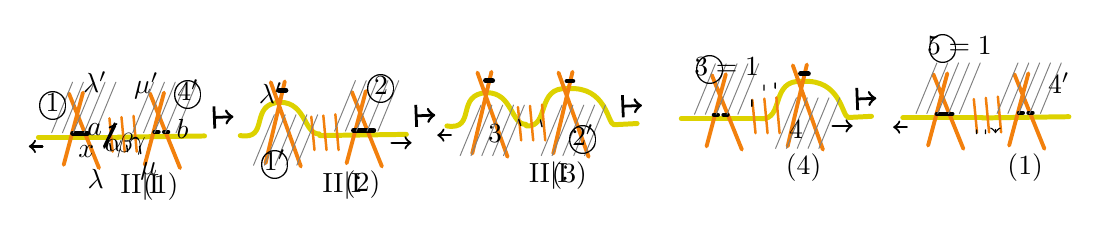
\begin{tikzpicture}[x=.0051cm,y=-.0051cm,line cap=round,line join=round]
\draw[yellow!70!olive,line width=1.8pt] (210,524)--(408,524);
\draw[yellow!70!olive,line width=1.8pt] (408,524)--(624,521);
\draw[orange!80!brown,line width=1.4pt] (286,415)--(361,601) (321,413)--(273,593);
\draw[orange!80!brown,line width=1.4pt] (488,415)--(563,601) (523,413)--(475,593);
\draw[black,line width=1.7pt] (295,514)--(333,514);\draw[black,dotted,line width=1.5pt] (499,511)--(543,511);
\draw[orange!80!brown,line width=.9pt] (387,477)--(395,560);
\draw[orange!80!brown,line width=.9pt] (417,474)--(425,560);
\draw[orange!80!brown,line width=.9pt] (447,471)--(455,560);
\draw[black,->,line width=.8pt] (220,547)--(186,547);
\draw[black,|->,line width=1pt] (645,475)--(696,473);
\node at (515,647) {(1)};
\draw[gray,line width=.35pt] (243,513)--(295,387);
\draw[gray,line width=.35pt] (270,513)--(322,387);
\draw[gray,line width=.35pt] (297,513)--(349,387);
\draw[gray,line width=.35pt] (324,513)--(376,387);
\draw[gray,line width=.35pt] (351,513)--(403,387);
\draw[gray,line width=.35pt] (445,513)--(497,387);
\draw[gray,line width=.35pt] (472,513)--(524,387);
\draw[gray,line width=.35pt] (499,513)--(551,387);
\draw[gray,line width=.35pt] (526,513)--(578,387);
\draw[gray,line width=.35pt] (553,513)--(605,387);
\node at (463,648) {$\deleted{\unsure{\mathrm{II}|\mathrm{I}}}$};
\draw[yellow!70!olive,line width=1.8pt] (713,520)..controls(788,532)and(733,440)..(813,437)..controls(877,438)and(872,517)..(910,516);
\draw[yellow!70!olive,line width=1.8pt] (911,520)--(1127,517);
\draw[orange!80!brown,line width=1.4pt] (789,387)--(864,597) (824,385)--(776,589);
\draw[orange!80!brown,line width=1.4pt] (991,411)--(1066,597) (1026,409)--(978,589);
\draw[black,line width=1.7pt] (809,407)--(827,407) (995,507)--(1046,507);
\draw[orange!80!brown,line width=.9pt] (890,473)--(898,556);
\draw[orange!80!brown,line width=.9pt] (920,470)--(928,556);
\draw[orange!80!brown,line width=.9pt] (950,467)--(958,556);
\draw[black,->,line width=.8pt] (1090,538)--(1140,538);
\draw[black,|->,line width=1pt] (1148,471)--(1199,469);
\node at (1018,643) {(2)};
\draw[gray,line width=.35pt] (746,594)--(798,468);
\draw[gray,line width=.35pt] (773,594)--(825,468);
\draw[gray,line width=.35pt] (800,594)--(852,468);
\draw[gray,line width=.35pt] (827,594)--(879,468);
\draw[gray,line width=.35pt] (854,594)--(906,468);
\draw[gray,line width=.35pt] (948,509)--(1000,383);
\draw[gray,line width=.35pt] (975,509)--(1027,383);
\draw[gray,line width=.35pt] (1002,509)--(1054,383);
\draw[gray,line width=.35pt] (1029,509)--(1081,383);
\draw[gray,line width=.35pt] (1056,509)--(1108,383);
\node at (966,644) {$\deleted{\unsure{\mathrm{II}|\mathrm{I}}}$};
\draw[yellow!70!olive,line width=1.8pt] (1228,496)..controls(1303,508)and(1248,416)..(1328,413)..controls(1392,414)and(1387,493)..(1425,492);
\draw[yellow!70!olive,line width=1.8pt] (1426,496)..controls(1486,500)and(1448,397)..(1530,403)..controls(1626,397)and(1628,490)..(1644,493)--(1702,490);
\draw[orange!80!brown,line width=1.4pt] (1304,363)--(1379,573) (1339,361)--(1291,565);
\draw[orange!80!brown,line width=1.4pt] (1506,363)--(1581,573) (1541,361)--(1493,565);
\draw[black,line width=1.7pt] (1324,383)--(1342,383) (1527,384)--(1542,384);
\draw[orange!80!brown,line width=.9pt] (1405,449)--(1413,532);
\draw[orange!80!brown,line width=.9pt] (1435,446)--(1443,532);
\draw[orange!80!brown,line width=.9pt] (1465,443)--(1473,532);
\draw[black,->,line width=.8pt] (1238,519)--(1204,519);
\draw[black,|->,line width=1pt] (1663,447)--(1714,445);
\node at (1533,619) {(3)};
\draw[gray,line width=.35pt] (1261,570)--(1313,444);
\draw[gray,line width=.35pt] (1288,570)--(1340,444);
\draw[gray,line width=.35pt] (1315,570)--(1367,444);
\draw[gray,line width=.35pt] (1342,570)--(1394,444);
\draw[gray,line width=.35pt] (1369,570)--(1421,444);
\draw[gray,line width=.35pt] (1463,570)--(1515,444);
\draw[gray,line width=.35pt] (1490,570)--(1542,444);
\draw[gray,line width=.35pt] (1517,570)--(1569,444);
\draw[gray,line width=.35pt] (1544,570)--(1596,444);
\draw[gray,line width=.35pt] (1571,570)--(1623,444);
\node at (1481,620) {$\deleted{\unsure{\mathrm{II}|\mathrm{I}}}$};
\draw[yellow!70!olive,line width=1.8pt] (1812,478)--(2010,478);
\draw[yellow!70!olive,line width=1.8pt] (2010,478)..controls(2070,482)and(2032,379)..(2114,385)..controls(2210,379)and(2212,472)..(2228,475)--(2286,472);
\draw[orange!80!brown,line width=1.4pt] (1888,369)--(1963,555) (1923,367)--(1875,547);
\draw[orange!80!brown,line width=1.4pt] (2090,345)--(2165,555) (2125,343)--(2077,547);
\draw[black,dotted,line width=1.5pt] (1893,468)--(1939,468);\draw[black,line width=1.7pt] (2109,366)--(2129,366);
\draw[orange!80!brown,line width=.9pt] (1989,431)--(1997,514);
\draw[orange!80!brown,line width=.9pt] (2019,428)--(2027,514);
\draw[orange!80!brown,line width=.9pt] (2049,425)--(2057,514);
\draw[black,->,line width=.8pt] (2189,496)--(2239,496);
\draw[black,|->,line width=1pt] (2247,429)--(2298,427);
\node at (2117,601) {(4)};
\draw[gray,line width=.35pt] (1845,467)--(1897,341);
\draw[gray,line width=.35pt] (1872,467)--(1924,341);
\draw[gray,line width=.35pt] (1899,467)--(1951,341);
\draw[gray,line width=.35pt] (1926,467)--(1978,341);
\draw[gray,line width=.35pt] (1953,467)--(2005,341);
\draw[gray,line width=.35pt] (2047,552)--(2099,426);
\draw[gray,line width=.35pt] (2074,552)--(2126,426);
\draw[gray,line width=.35pt] (2101,552)--(2153,426);
\draw[gray,line width=.35pt] (2128,552)--(2180,426);
\draw[gray,line width=.35pt] (2155,552)--(2207,426);
\draw[yellow!70!olive,line width=1.8pt] (2364,476)--(2562,476);
\draw[yellow!70!olive,line width=1.8pt] (2562,476)--(2778,473);
\draw[orange!80!brown,line width=1.4pt] (2440,367)--(2515,553) (2475,365)--(2427,545);
\draw[orange!80!brown,line width=1.4pt] (2642,367)--(2717,553) (2677,365)--(2629,545);
\draw[black,line width=1.7pt] (2449,466)--(2487,466);\draw[black,dotted,line width=1.5pt] (2653,463)--(2697,463);
\draw[orange!80!brown,line width=.9pt] (2541,429)--(2549,512);
\draw[orange!80!brown,line width=.9pt] (2571,426)--(2579,512);
\draw[orange!80!brown,line width=.9pt] (2601,423)--(2609,512);
\draw[black,->,line width=.8pt] (2374,499)--(2340,499);
\node at (2669,599) {(1)};
\draw[gray,line width=.35pt] (2397,465)--(2449,339);
\draw[gray,line width=.35pt] (2424,465)--(2476,339);
\draw[gray,line width=.35pt] (2451,465)--(2503,339);
\draw[gray,line width=.35pt] (2478,465)--(2530,339);
\draw[gray,line width=.35pt] (2505,465)--(2557,339);
\draw[gray,line width=.35pt] (2599,465)--(2651,339);
\draw[gray,line width=.35pt] (2626,465)--(2678,339);
\draw[gray,line width=.35pt] (2653,465)--(2705,339);
\draw[gray,line width=.35pt] (2680,465)--(2732,339);
\draw[gray,line width=.35pt] (2707,465)--(2759,339);
\node at (350,505) {$a$};\node at (569,503) {$b$};\node at (351,387) {$\lambda^{\prime}$};\node at (479,396) {$\mu^{\prime}$};\node at (353,629) {$\lambda$};\node at (485,609) {$\mu$};
\node at (245,448) {\textcircled{1}};\node at (583,417) {\textcircled{$4^{\prime}$}};\node at (799,590) {\textcircled{$1^{\prime}$}};\node at (1064,406) {\textcircled{2}};\node at (1348,516) {$3$};\node at (1567,529) {\textcircled{$2^{\prime}$}};\node at (1925,358) {\textcircled{$3=1$}};\node at (2098,504) {$4$};\node at (2505,306) {\textcircled{$5=1$}};\node at (2753,389) {$4^{\prime}$};
\node at (329,560) {$x$};\node at (397,546) {$\alpha$};\node at (427,546) {$\beta$};\node at (458,546) {$\unsure{\gamma}$};\node at (789,415) {$\unsure{\lambda^{\prime}}$};
\draw[black,->,line width=.5pt] (388,540)--(391,557) (430,544)--(432,560) (462,547)--(465,565) (1407,480)--(1412,495) (1461,481)--(1465,498) (1988,447)--(1988,431) (2018,407)--(2018,394) (2046,402)--(2046,389) (2548,506)--(2548,515) (2570,506)--(2570,515) (2595,505)--(2595,514);
\draw[black,line width=.6pt] (373,547)--(400,489) (374,551)--(402,496) (387,500)--(405,491);
\end{tikzpicture}}
\uline{NB} Pour chaque position $(D,a,\omega)$ dans le cycle, on a indiqué en pointillé l'arc de
transition $b$ qui suit \unsure{$a$} suivant l'orientation $-\omega$.

Il faudrait regarder à part le cas où on part avec un arc de \deleted{transition}\inserted{spécialisation},
exceptionnel, correspondant à un balayage de couloir. Il ne devrait pas y
avoir de différence.

\margin{\diagram{\begin{array}{r}\text{arcs de spécialisation}\\\text{arcs de généralisation}\end{array}\left\}\vphantom{\begin{array}{r}1\\2\end{array}}\right.\ \text{arcs de transition}}}
\margin{\uline{arcs \deleted{\unsure{de combinatoire}}\inserted{d'isomorphie}}}

\margin{$\geq \unsure{\nu|r}-2+(2\unsure{+|,}2)=2\unsure{\nu|r}+2$\\dont}
\figure{\begin{tikzpicture}[x=.006cm,y=-.006cm,line cap=round,line join=round]
\draw[yellow!70!olive,line width=1.8pt] (256,1577)--(840,1536) (400,1410)--(590,1404) (400,1410)..controls(483,1493)and(542,1517)..(647,1542) (397,1559)--(592,1407);
\draw[orange!80!brown,line width=1.4pt] (368,1322)--(468,1646) (423,1306)--(360,1630) (563,1307)--(671,1644) (617,1295)--(553,1652);
\draw[black,dashed,line width=1.8pt] (399,1410)--(591,1405) (400,1410)..controls(488,1504)and(534,1501)..(574,1533) (450,1556)--(590,1407) (385,1565)--(572,1550);
\draw[black,->,line width=.8pt] (410,1422)--(459,1469) (310,1599)--(254,1599) (709,1562)--(775,1562);
\draw[gray,line width=.35pt] (396,1418)--(344,1480) (409,1436)--(371,1506) (443,1470)--(412,1514);
\node at (367,1409) {$\unsure{x^{\prime}|z^{\prime}}$};\node at (625,1394) {$y^{\prime}$};\node at (349,1584) {$x$};\node at (669,1569) {$y$};\node at (472,1532) {$\unsure{o}$};
\draw[yellow!70!olive,line width=1.8pt] (947,1568)--(1410,1553) (1041,1421)..controls(1077,1420)and(1083,1539)..(1100,1551)--(1207,1551);
\draw[orange!80!brown,line width=1.4pt] (1008,1318)--(1103,1641) (1074,1296)--(992,1664) (1217,1298)--(1335,1665) (1278,1273)--(1218,1637);
\draw[black,dashed,line width=1.6pt] (1043,1421)..controls(1075,1423)and(1084,1537)..(1100,1550) (1100,1550)--(1216,1542)..controls(1235,1463)and(1225,1418)..(1251,1405);
\draw[black,line width=1.4pt] (1212,1443)..controls(1223,1418)and(1231,1411)..(1251,1405) (1008,1564)--(1279,1555);
\foreach \x in {1012,1026,1040,1054,1068,1082,1096,1110,1124,1138,1152,1166,1180,1194,1208,1222,1236,1250,1264}{\draw[black,line width=.4pt] (\x,1557)--++(9,-12);}
\node at (1010,1419) {$z$};\node at (1286,1386) {$t$};\node at (988,1584) {$x$};\node at (1328,1584) {$y$};\node at (933,1637) {$(3)$};
\draw[yellow!70!olive,line width=1.8pt] (811,1738)--(1074,1729)--(1078,1912)--(816,1922)--cycle;
\draw[orange!80!brown,line width=1.4pt] (941,1827)--(811,1738) (941,1827)--(893,1734) (941,1827)--(942,1734) (941,1827)--(991,1732) (941,1827)--(1074,1729) (941,1827)--(1075,1792) (941,1827)--(1077,1827) (941,1827)--(1077,1862) (941,1827)--(1078,1912) (941,1827)--(977,1917) (941,1827)--(941,1918) (941,1827)--(905,1919) (941,1827)--(816,1922) (941,1827)--(815,1849) (941,1827)--(814,1812) (941,1827)--(813,1787);
\fill[black] (941,1827) circle (7);
\draw[black,->,line width=1pt] (814,1740)--(860,1773) (896,1736)--(912,1771) (944,1738)--(946,1770) (991,1735)--(978,1773) (1072,1730)--(1027,1764) (1072,1794)--(1034,1804) (1074,1824)--(1040,1825) (1074,1859)--(1035,1846) (1075,1908)--(1040,1876) (975,1914)--(962,1878) (940,1915)--(941,1879) (906,1918)--(918,1881) (818,1916)--(859,1884) (861,1843)--(815,1849) (858,1815)--(813,1813) (857,1801)--(813,1787);
\node at (782,1735) {$y^{\prime}$};\node at (1095,1729) {$x^{\prime}$};\node at (794,1942) {$x$};\node at (1094,1923) {$y$};
\node at (895,1705) {$\unsure{\gamma|\delta}$};\node at (944,1704) {$\beta$};\node at (1005,1705) {$\alpha$};\node at (1095,1792) {$\alpha$};\node at (1108,1828) {$\beta$};\node at (1101,1861) {$\unsure{\gamma|\delta}$};\node at (978,1945) {$\unsure{\gamma|\delta}$};\node at (945,1948) {$\beta$};\node at (901,1945) {$\alpha$};\node at (782,1787) {$\unsure{\gamma|\delta}$};\node at (782,1819) {$\beta$};\node at (782,1854) {$\alpha$};
\node at (838,1754) {$\mu$};\node at (1046,1768) {$\lambda$};\node at (1038,1880) {$\mu^{\prime}$};\node at (858,1881) {$\unsure{\lambda^{\prime}}$};\node at (1184,1842) {$(2)$};\node at (940,2003) {$(1)$};
\draw[yellow!70!olive,line width=1.7pt] (317,1781)--(548,1759)--(549,1944)--(318,1958)--cycle (154,1630)--(242,1620)--(249,1698)--(181,1710) (162,1702)--(154,1630) (595,1596)--(616,1676)--(713,1652) (596,1588)--(695,1567)--(743,1642) (153,2031)--(263,2030)--(270,2147)--(134,2142)--cycle (616,2023)--(754,2001) (768,2024)--(774,2149) (617,2030)--(616,2134)--(753,2153);
\draw[green!25!black,line width=2.5pt] (250,1699)--(306,1776) (551,1756)--(616,1678) (320,1959)--(253,2027) (548,1942)--(617,2020);
\draw[orange!80!brown,line width=1.2pt] (273,1648)--(199,1828) (174,1804)--(307,1774)..controls(344,1756)and(350,1724)..(374,1719) (585,1636)--(657,1780) (520,1744)--(689,1786) (223,1876)--(255,2027) (190,1907)--(320,1957) (656,1836)--(594,2083) (512,1963)..controls(564,1918)and(616,1910)..(691,1888);
\draw[black,line width=.8pt] (320,1957)--(448,1850)--(551,1758) (306,1774)..controls(336,1768)and(348,1735)..(375,1722) (478,1799)--(519,1714) (552,1743)--(548,1758) (248,1701)--(302,1773) (316,1876)..controls(378,1871)and(402,1854)..(448,1850) (449,1850)--(548,1851) (322,1955)..controls(353,1899)and(373,1884)..(448,1850) (448,1850)..controls(481,1816)and(512,1784)..(550,1759);
\fill[black] (318,1876) circle (6);\draw[black] (450,1850) circle (5);\draw[black] (465,1844) circle (4);
\foreach \x in {380,401,421,439,460,480}{\draw[black!65,line width=.45pt] (\x,1778)--(448,1850)--(\x,1951);}
\foreach \y in {1790,1803,1816,1829,1842,1855,1868,1881,1894,1907,1920,1933,1946}{\draw[black!65,line width=.45pt] (319,\y)--(448,1850)--(548,\y);}
\draw[black,->,line width=.9pt] (321,1869)--(400,1857) (545,1854)--(478,1853) (381,1777)--(381,1833)--(420,1844) (377,1948)--(378,1893) (544,1790)--(513,1793)--(496,1813);
\draw[black,line width=.5pt] (331,1812)--(319,1808)--(351,1823) (342,1836)--(367,1832) (331,1909)--(369,1889) (524,1885)--(545,1895) (504,1905)--(543,1911);
\draw[gray,line width=.4pt] (237,1709)--(270,1772)--(272,1903)--(351,2072) (258,2029)..controls(291,2056)and(361,2078)..(435,2116) (260,2042)..controls(349,2120)and(377,2076)..(438,2116) (263,2054)..controls(332,2114)and(379,2094)..(409,2128) (550,1951)..controls(535,2018)and(515,2048)..(476,2083) (553,1935)--(572,1965) (566,1944)--(584,1972) (577,1953)--(593,1981);
\node at (300,1747) {$y^{\prime}$};\node at (563,1735) {$x^{\prime}$};\node at (298,1993) {$\unsure{x}$};\node at (569,1980) {$\unsure{y}$};\node at (376,1742) {$\unsure{\gamma|\theta}$};\node at (433,1739) {$\beta$};\node at (489,1734) {$\alpha$};\node[draw,ellipse] at (448,1696) {$\unsure{3}$};
\node at (572,1800) {$\alpha$};\node at (574,1855) {$\beta$};\node at (575,1900) {$\unsure{\gamma}$};\node at (386,1986) {$\alpha$};\node at (435,1990) {$\beta$};\node at (482,1987) {$\unsure{\gamma}$};\node at (282,1825) {$\unsure{\gamma}$};\node at (282,1886) {$\beta$};\node at (281,1940) {$\alpha$};\node at (678,1875) {$(4)$};\node at (469,2034) {$(1)$};\node at (447,1874) {$\unsure{o}$};
\draw[yellow!70!olive,line width=1.7pt] (1116,2024)--(1308,2015)--(1329,2164)--(1118,2174)--cycle;
\draw[gray,->,line width=.4pt] (1299,2026)--(1261,2069) (1123,2167)--(1174,2134) (1324,2157)--(1271,2135);
\node at (1338,2006) {$x^{\prime}$};\node at (1108,2191) {$x$};\node at (1339,2190) {$y$};\node at (1171,2121) {$\lambda$};\node at (1250,2121) {$\mu$};
\draw[yellow!70!olive,line width=1.7pt] (1660,1506)--(1691,1501)--(1723,1363)--(1810,1331)..controls(1840,1299)and(1873,1282)..(1914,1298) (1961,1304)..controls(2021,1288)and(2007,1356)..(2042,1422)--(2055,1471)--(2098,1466);
\draw[orange!80!brown,line width=1.1pt] (1654,1369)..controls(1660,1494)and(1716,1634)..(1761,1740) (1705,1347)--(1613,1736) (2105,1314)--(1971,1738) (2019,1282)..controls(2042,1396)and(2103,1601)..(2136,1719) (1705,1347)--(1811,1309) (1837,1304)--(1837,1384) (1837,1304)..controls(1885,1243)and(1896,1268)..(1941,1281)..controls(1961,1225)and(1986,1277)..(2019,1282) (1837,1304)--(1847,1774) (1882,1263)--(1925,1756) (1940,1281)--(1946,1776) (1634,1573)--(1713,1655) (1678,1634)--(1765,1650) (1786,1645)--(1870,1685)--(1966,1643);
\draw[orange!80!brown,line width=1.1pt] (1412,1820)--(1493,2073) (1494,1758)--(1387,2078) (1640,1800)--(1722,2092) (1705,1780)--(1628,2101) (1531,1756)--(1530,2056) (1571,1755)--(1583,2058) (1600,1757)--(1613,2069) (1517,1770)--(1540,1755) (1556,1757)--(1585,1758) (1591,1755)--(1615,1760);
\draw[orange!80!brown,line width=1.1pt] (1964,1853)--(2066,2001) (2043,1822)--(1963,2037) (2437,1790)--(2573,1950) (2552,1781)--(2442,1989) (2154,1744)--(2162,2014) (2208,1740)--(2222,2018) (2264,1733)--(2274,2016) (2331,1748)--(2334,1996);
\draw[orange!80!brown,line width=1.3pt] (2144,1792)--(2164,1791) (2196,1796)--(2226,1796) (2256,1791)--(2280,1790) (2322,1789)--(2340,1789) (2155,1987)--(2170,1987) (2214,1992)--(2233,1992) (2267,1991)--(2283,1991) (2326,1984)--(2342,1984);
\draw[yellow!70!olive,line width=1.7pt] (1957,1925)..controls(1989,1922)and(1970,1986)..(2053,1934) (1957,1925)..controls(2174,1927)and(2334,1917)..(2437,1904)..controls(2476,1937)and(2500,1908)..(2570,1887);
\draw[green!20!black,line width=3pt,->] (2004,1923)..controls(2211,1929)and(2398,1902)..(2564,1888);
\draw[green!20!black,line width=2.5pt] (2024,1954)--(2056,1932);
\foreach \x in {2114,2125,2136,2155,2182,2203,2224,2246,2267,2287,2307,2328,2348,2371,2391,2412}{\draw[black,line width=.4pt] (\x,1904)--++(8,-12);}
\draw[gray,line width=.45pt] (2039,1815)..controls(2125,1707)and(2378,1704)..(2443,1777) (2151,1714)--(2454,1752);
\draw[black,->,line width=.4pt] (2227,1651)--(2222,1779) (2233,1648)--(2240,1778);
\node at (2244,1617) {$\unsure{\nu-2|r-2}$};\node at (2011,2078) {$2$};\node at (2501,2039) {$2$};
\draw[black,line width=.5pt] (2156,2034)..controls(2170,2058)and(2240,2028)..(2254,2063)..controls(2256,2045)and(2350,2055)..(2347,2026);
\node at (2260,2093) {$\unsure{\nu|r}$};
\draw[orange!70!brown,line width=.4pt] (2187,2121)..controls(2444,2125)and(2724,2201)..(2881,2210);
\end{tikzpicture}}

\margin{104}
